% Created 2023-10-27 Fri 11:08
% Intended LaTeX compiler: pdflatex
\documentclass[presentation]{beamer}
\usepackage[utf8]{inputenc}
\usepackage[T1]{fontenc}
\usepackage{graphicx}
\usepackage{longtable}
\usepackage{wrapfig}
\usepackage{rotating}
\usepackage[normalem]{ulem}
\usepackage{amsmath}
\usepackage{amssymb}
\usepackage{capt-of}
\usepackage{hyperref}
\usepackage{graphicx, hyperref, url}
\mode<beamer>{\usetheme{Madrid}}
\usetheme{default}
\author{Rafael Castro}
\date{27/10/2023}
\title{How to Use Mathematics to Write Better Programs}
\hypersetup{
 pdfauthor={Rafael Castro},
 pdftitle={How to Use Mathematics to Write Better Programs},
 pdfkeywords={},
 pdfsubject={},
 pdfcreator={Emacs 28.2 (Org mode 9.7)}, 
 pdflang={English}}
\begin{document}

\maketitle
\section{Introduction}
\label{sec:orga8a9892}
\begin{frame}[label={sec:org21ee3d2}]{Bugs are annoying}
\begin{center}

\includegraphics[width=0.8\textwidth]{./blue_screem_new.png}
\end{center}
\end{frame}
\begin{frame}[label={sec:orge856d8f}]{Bugs are annoying}
\begin{center}
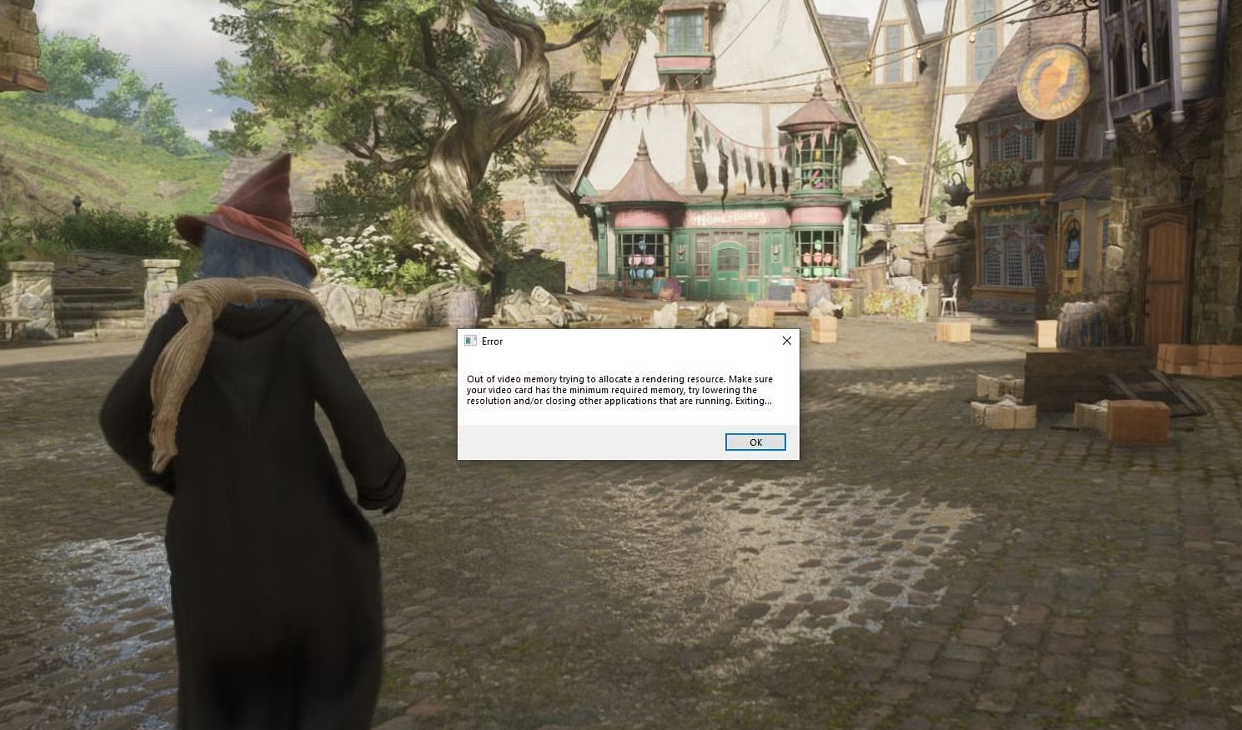
\includegraphics[width=0.8\textwidth]{./harry.png}
\end{center}
\end{frame}
\section{Software bugs are catastrophic}
\label{sec:orgb8c2f33}
\begin{frame}[label={sec:org90f989a}]{Therac-25: The killing radiation therapy machine}
\begin{center}
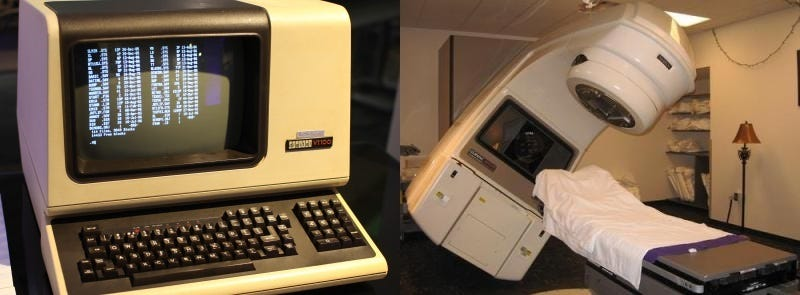
\includegraphics[width=.9\linewidth]{./therac25.png}
\end{center}
\end{frame}
\begin{frame}[label={sec:org2d9b594}]{People got hurt}
\begin{itemize}
\item At least 6 accidents between 1985 and 1987, 3 died later
\end{itemize}

\begin{center}
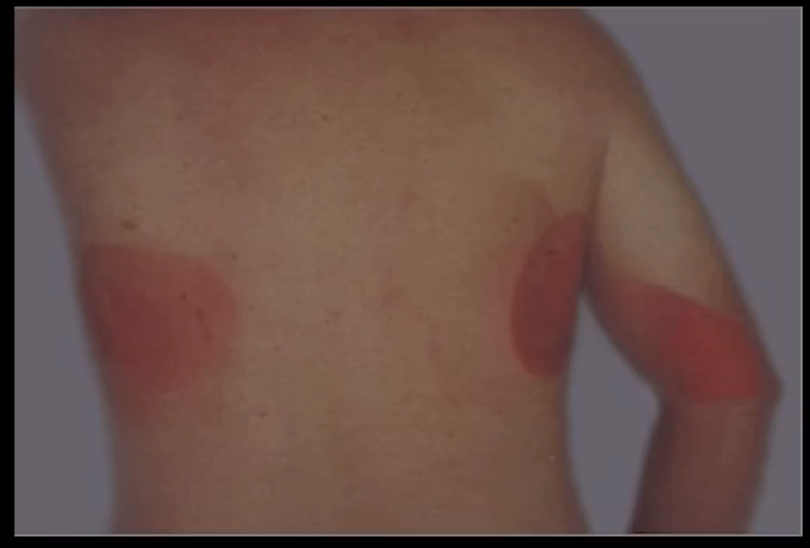
\includegraphics[width=0.6\textwidth]{./radiation.png}
\end{center}
\end{frame}
\begin{frame}[label={sec:org992ff53}]{Malfunction messages}
\begin{itemize}
\item Malfunction messages from 1 to 64, with no extra information
\end{itemize}

\begin{center}

\includegraphics[width=0.8\textwidth]{./error54.png}
\end{center}
\end{frame}
\begin{frame}[label={sec:orgb3b33c2}]{The machine a bug}
\begin{itemize}
\item The machine had three modes: field light, direct electron beam, x-ray
\end{itemize}

\begin{center}
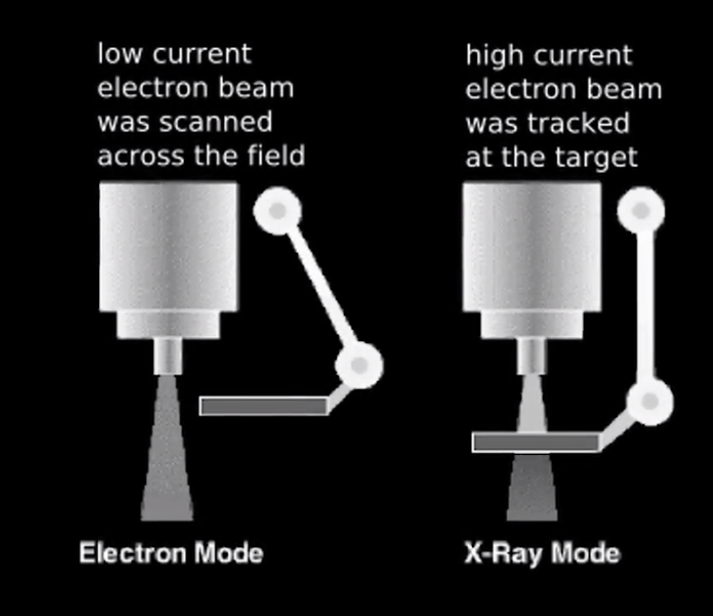
\includegraphics[width=0.6\textwidth]{./beam.png}
\end{center}
\end{frame}
\begin{frame}[label={sec:org8b12509}]{The machine a bug}
\begin{center}
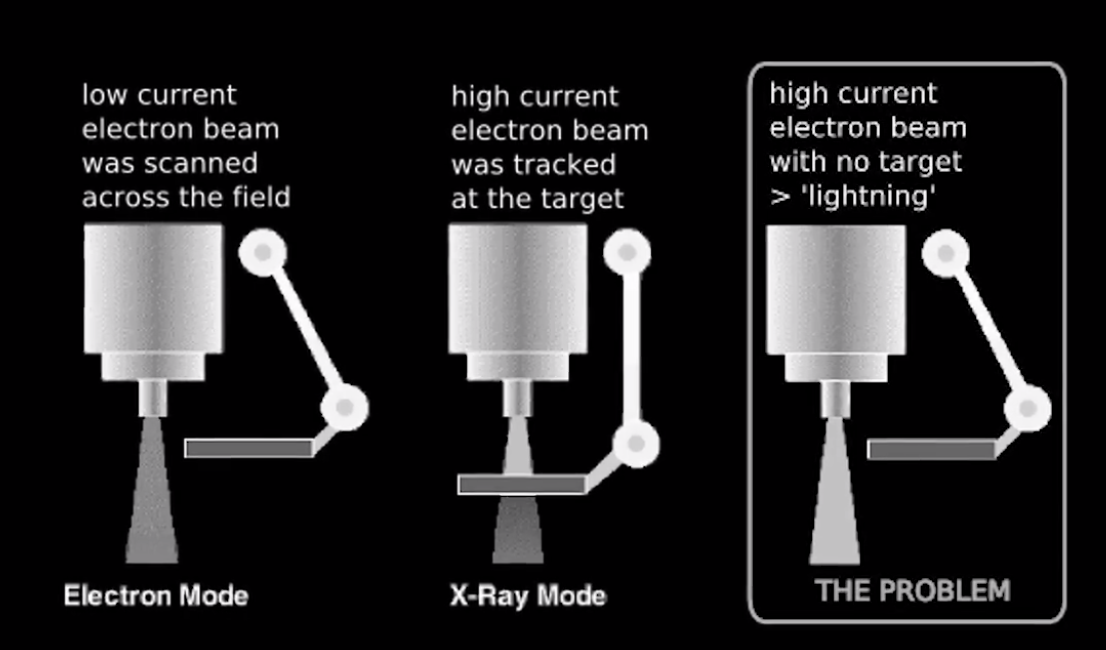
\includegraphics[width=0.7\textwidth]{./change.png}
\end{center}
\end{frame}
\begin{frame}[label={sec:orgb7c6d77}]{How to cause the bug}
\begin{center}
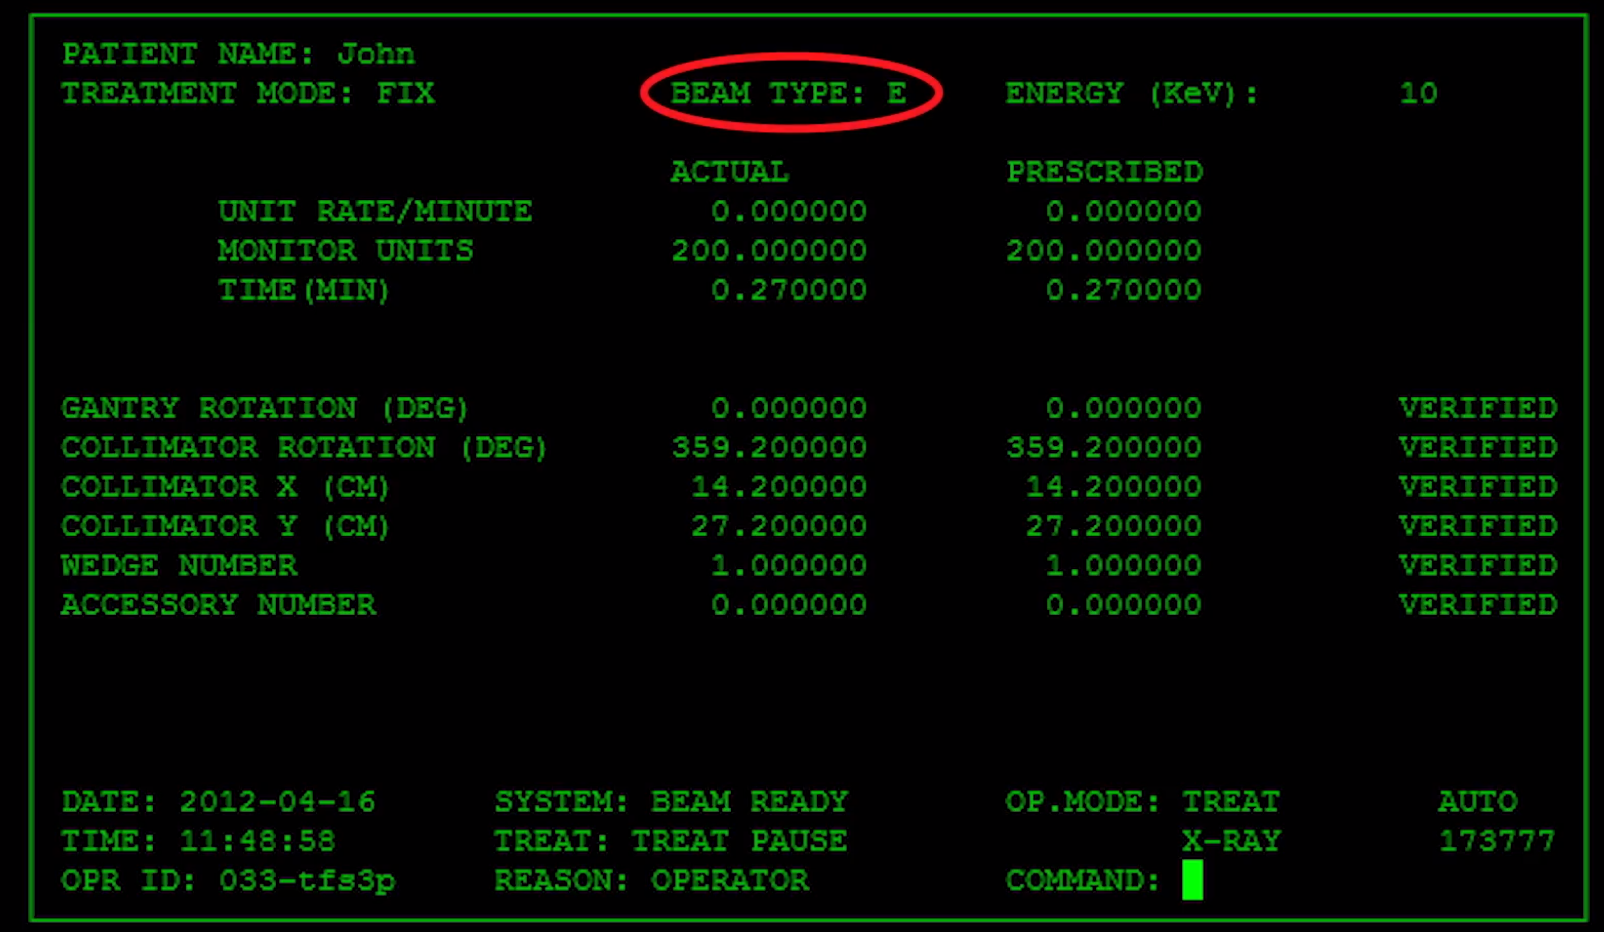
\includegraphics[width=0.8\textwidth]{./mistake.png}
\end{center}
\end{frame}
\section{Formal Methods}
\label{sec:org3cba742}
\begin{frame}[label={sec:orgd1a428f}]{How to write software that don't cause catastrophic failures?}
\begin{itemize}
\item Formal Methods!
\item There are many techniques: static analysis, model checking and formal proving
\end{itemize}
\end{frame}
\begin{frame}[label={sec:orge7953b0}]{What is to prove something?}
\begin{itemize}
\item Establishing mathematical facts that are universally true
\item You know some: Pythoragoras theorem: \(\forall a b c. c^2 = a^2 + b^2\)
\end{itemize}
\begin{center}
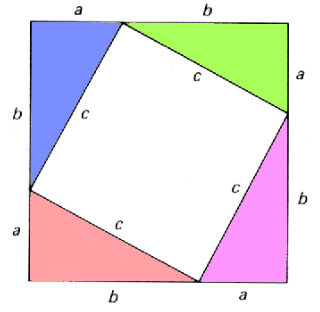
\includegraphics[width=0.2\textwidth]{./pythagoras.png}
\end{center}

Two ways to calculate this area:
\begin{enumerate}
\item \((a + b)(a + b) = a^2 + ab + ab + b^2\)
\item \(4(ab)/2 + c^2\)

they should be the same!

\(a^2 + ab + ab + b^2 = 4(ab)/2 + c^2\)

\(a^2 + b^2 = c^2\)

\item How can you be sure that there is no mistake in the proof?
\end{enumerate}
\end{frame}
\begin{frame}[label={sec:orga738dca}]{Proof assistants}
\begin{itemize}
\item Proof assistants: programs that verify if your proof is correct!
\begin{itemize}
\item We trust the verifier!
\end{itemize}

\item I use a proof assistant called Isabelle/HOL to verify programs
\item How my research works:
\begin{enumerate}
\item I write a specification of the program: what it should do, and what it should \alert{not} do
\item I write the program
\item I write a proof that the program respects the specification
\begin{itemize}
\item Usually this requires writing many other auxiliary proofs
\end{itemize}
\end{enumerate}
\end{itemize}
\end{frame}
\begin{frame}[label={sec:orge6e44df}]{Examples!}
\begin{itemize}
\item Pythagoras
\item Sorting
\end{itemize}
\end{frame}
\begin{frame}[label={sec:org1256b7e}]{This is a real job!}
\begin{itemize}
\item TLA+/TLC: Amazon AWS, Intel, Microsoft\ldots{}
\item Coq (CompCert): Airbus
\item Isabelle/HOL (seL4): Defense Advanced Research Projects Agency (DARPA)
\item Formal methods companies: Absint, Trustworthy Systems
\item Apple: \url{https://jobs.apple.com/en-us/details/200343072/formal-verification-engineer}
\end{itemize}
\end{frame}
\begin{frame}[label={sec:org3279d51}]{Thank you!}
\begin{itemize}
\item Questions?
\end{itemize}
\end{frame}
\end{document}